\section{Installation and First Steps: Double Link List}

\subsection{Step 01: Install Enterprise Architect}
$\blacktriangleright$ Download and install EA\\
Go to http://www.sparxsystems.com.au/ to get a free 30 day trial.
\begin{figure}[!h]
	\centering
  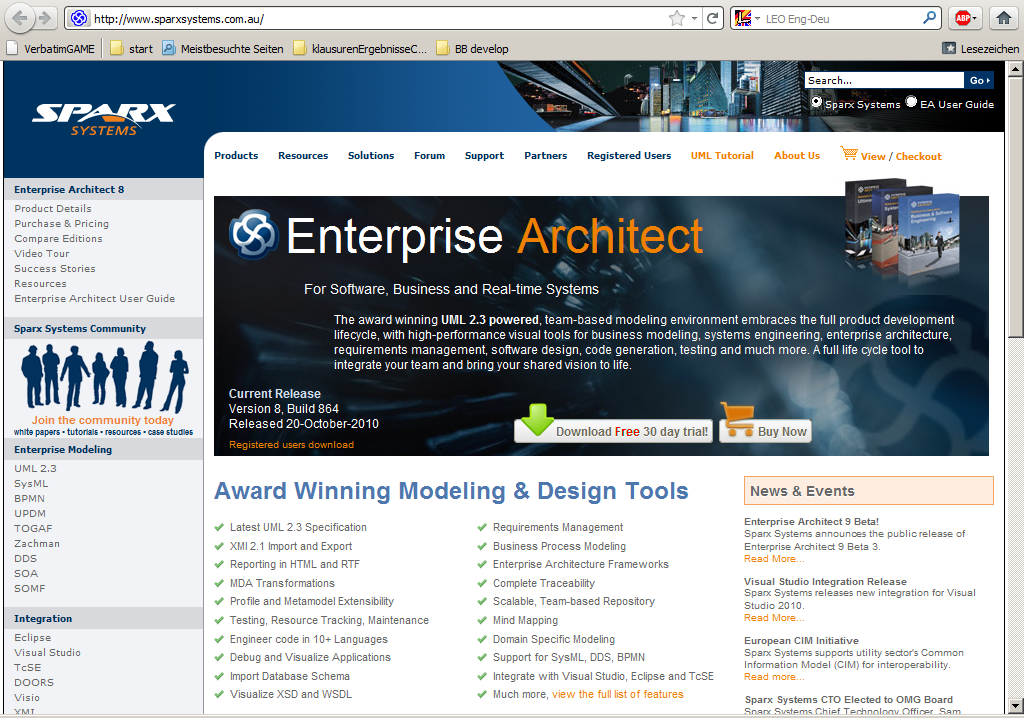
\includegraphics[width=0.5\textwidth]{pics/ea_download.png}
	\caption{Enterprise Architect Homepage}
\end{figure}

$\blacktriangleright$ Install our EA-Plugin\\
Go to
\url{http://www.moflon.org/fileadmin/download/moflon-ide/eclipse-plugin/ea-ecore-addin/ea-ecore-addin.zip}
Just unpack the ZIP-File, run setup.exe and follow the instructions.

\begin{figure}[!h]
	\centering
  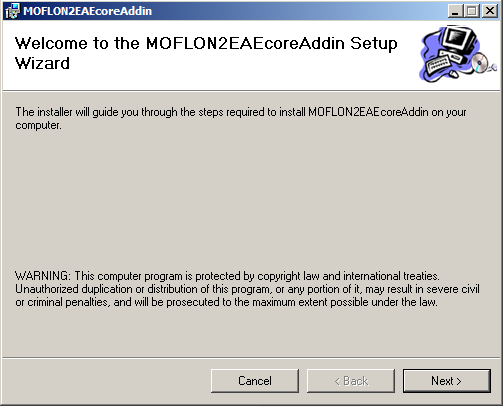
\includegraphics[width=0.3\textwidth]{pics/eaplugin_install.png}
	\caption{EA-Plugin Wizard}
\end{figure}

\subsection{Step 02: Install Eclipse}
$\blacktriangleright$ Install the latest version of JAVA (JDK).\\ %WO? bild ?
%URL! online tutorial

$\blacktriangleright$ Download the modeling Package ``Eclipse Modeling Tools
(includes Incubating components)''\\
http://www.eclipse.org/downloads/packages/eclipse-modeling-tools-includes-incubating-components/heliossr2\\
\begin{figure}[!h]
	\centering
  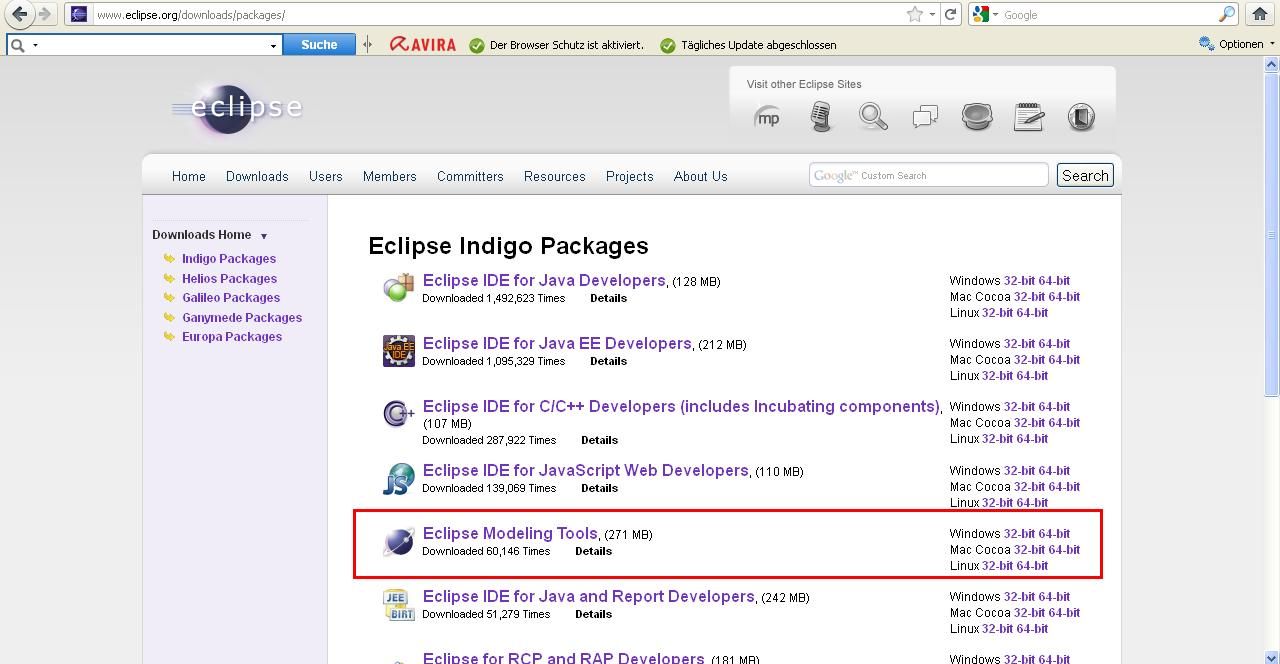
\includegraphics[width=0.5\textwidth]{pics/eclipse_modelingpackage.png}
	\caption{Download Modeling Package}
\end{figure}

$\blacktriangleright$ Download and install Eclipse.\\
For a detailed tutorial on how to install Eclipse and Eclipse Plugins please
refer to http://www.vogella.de/articles/Eclipse/article.html\\
(Tested for Windows 32bit, 64bit should work as well)\\

$\blacktriangleright$ Install our Eclipse Plugin.\\
%in eclipse BILD BILD
http://www.moflon.org/fileadmin/download/moflon-ide/eclipse-plugin/update-site2\\
Please note: Calculating requirements and dependencies when installing the
plugin might take quite a while depending on your internet connection! 

\subsection{Step 03: Try out our demo}
$\blacktriangleright$ Start eclipse with a workspace of your choice.\\

$\blacktriangleright$ Go to Window/Open Perspective/Other\ldots and choose
Moflon.\\

$\blacktriangleright$ In the toolbar a new action set should have appeared\ldots
Choose ``New Metamodel''.\\
\begin{figure}[!h]
	\centering
  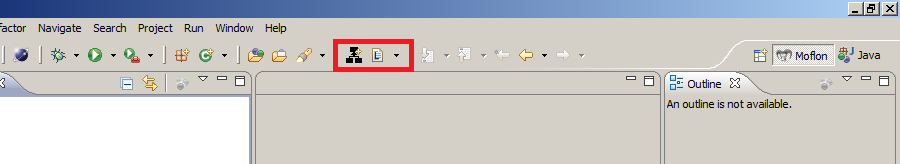
\includegraphics[width=0.8\textwidth]{pics/eclipse_metamodelButton.png}
	\caption{Eclipse New Metamodel}
\end{figure}

\subsection{Step 04: }
\subsection{Step 05: }
\subsection{Step 06: }
\subsection{Step 07: }
\subsection{Step 08: }
\subsection{Step 09: }
\subsection{Step 10: }
\subsection{Step 11: }
